\documentclass{beamer}
\usetheme{Rochester}
\usepackage{tcolorbox}
\tcbuselibrary{listings}
\usepackage{inconsolata}

\geometry{paperwidth = 4.75in, paperheight = 4.75in}

% Custom U of C color palette
\definecolor{ucMaroon}{RGB}{128,0,0}
\definecolor{ucDarkGray}{RGB}{118,118,118}
\definecolor{ucLightGray}{RGB}{214,214,206}

\setbeamercolor{block title}{fg=white,bg=ucMaroon}
\setbeamercolor{block title alerted}{use=alerted text,fg=white,bg=alerted text.fg}
\setbeamercolor{block title example}{use=example text,fg=white,bg=example text.fg}
\setbeamercolor{block body}{parent=normal text,use=block title,bg=ucLightGray}
\setbeamercolor{block body alerted}{parent=normal text,use=block title alerted,bg=block title alerted.bg}
\setbeamercolor{block body example}{parent=normal text,use=block title example,bg=block title example.bg}

\setbeamercolor{palette primary}{fg=white,bg=ucMaroon}
\setbeamercolor{palette secondary}{fg=white,bg=ucLightGray}
\setbeamercolor{palette tertiary}{fg=white,bg=ucDarkGray}
\setbeamercolor{palette quaternary}{fg=white,bg=black}

\setbeamercolor{sidebar}{bg=ucMaroon}

\setbeamercolor{palette sidebar primary}{fg=ucMaroon}
\setbeamercolor{palette sidebar secondary}{fg=white}
\setbeamercolor{palette sidebar tertiary}{fg=ucMaroon}
\setbeamercolor{palette sidebar quaternary}{fg=white}

\setbeamercolor{titlelike}{parent=palette primary}
\setbeamercolor{itemize item}{fg=ucMaroon}

% Code block formatting. Fragile frames needed for these to work.
\newtcblisting{gitCommand}{
  colframe=black,
  colback=ucLightGray,
  boxrule=1pt,
  arc=2pt,
  left=6pt,
  right=6pt,
  top=6pt,
  bottom=6pt,
  before=\vspace{6pt},
  boxsep=0pt,
  listing only,
  hbox
}


\title{Intermediate Git}
\subtitle{Day 4: Collaborating on GitHub}
\author{Raman A.~Shah}
\date{}

\begin{document}

%% Title
\begin{frame}[plain]
  \titlepage
  \footnotesize{Copyright (c) 2015 by Raman A.~Shah.\\
  \href{https://creativecommons.org/licenses/by-nc-sa/3.0/legalcode}
       {Creative Commons BY-NC-SA 3.0 Unported}.\\
   \href{https://github.com/ramanshah/intermediate\_git}
        {https://github.com/ramanshah/intermediate\_git}}
\end{frame}

%% Everyone's on master
\begin{frame}{Everyone's on master}
  \begin{figure}
    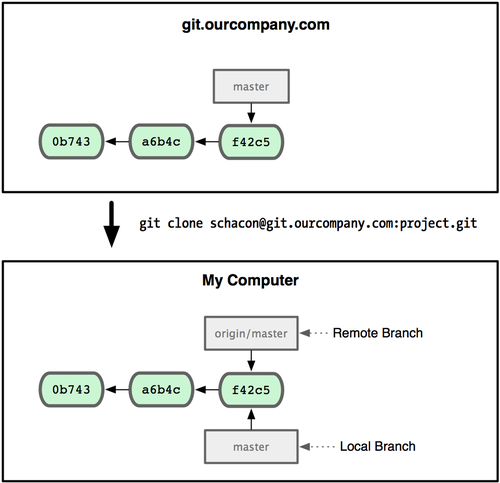
\includegraphics[scale=0.8]{18333fig0322-tn.png}
    \\ A standard \texttt{git clone}.
  \end{figure}
  \footnotesize{Scott Chacon,
    \emph{Pro Git},
    Fig.~3-22.
    \href{https://creativecommons.org/licenses/by-nc-sa/3.0/legalcode}{CC-BY-NC-SA}.
    \href{https://progit.org/}{https://progit.org/}}
\end{frame}

\begin{frame}{Everyone's on master}
  \begin{figure}
    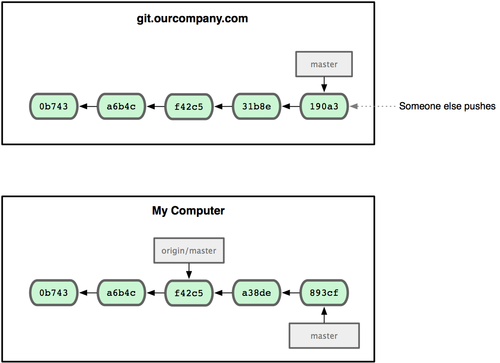
\includegraphics[scale=0.8]{18333fig0323-tn.png}
    \\ Local \texttt{master} has diverged from \texttt{origin/master}.
  \end{figure}
  \footnotesize{Scott Chacon,
    \emph{Pro Git},
    Fig.~3-23.
    \href{https://creativecommons.org/licenses/by-nc-sa/3.0/legalcode}{CC-BY-NC-SA}.
    \href{https://progit.org/}{https://progit.org/}}
\end{frame}

\begin{frame}{Everyone's on master}
  \begin{figure}
    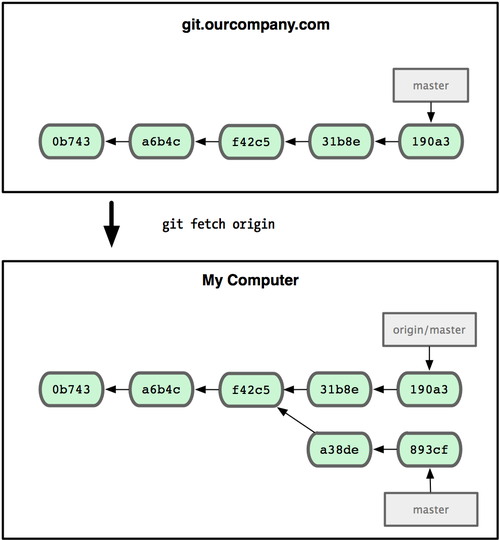
\includegraphics[scale=0.8]{18333fig0324-tn.png}
    \\ You have to \texttt{git fetch}, not \texttt{git pull}.
  \end{figure}
  \footnotesize{Scott Chacon,
    \emph{Pro Git},
    Fig.~3-24.
    \href{https://creativecommons.org/licenses/by-nc-sa/3.0/legalcode}{CC-BY-NC-SA}.
    \href{https://progit.org/}{https://progit.org/}}
\end{frame}

\begin{frame}{Everyone's on master}
  \begin{figure}
    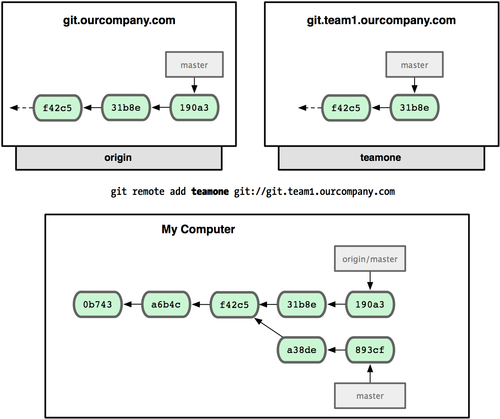
\includegraphics[scale=0.8]{18333fig0325-tn.png}
    \\ You can add a second remote.
  \end{figure}
  \footnotesize{Scott Chacon,
    \emph{Pro Git},
    Fig.~3-25.
    \href{https://creativecommons.org/licenses/by-nc-sa/3.0/legalcode}{CC-BY-NC-SA}.
    \href{https://progit.org/}{https://progit.org/}}
\end{frame}

\begin{frame}{Everyone's on master}
  \begin{figure}
    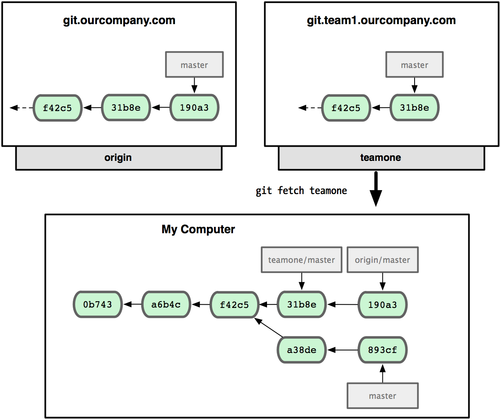
\includegraphics[scale=0.8]{18333fig0326-tn.png}
    \\ Again, \texttt{git fetch}, not \texttt{git pull}, is appropriate.
  \end{figure}
  \footnotesize{Scott Chacon,
    \emph{Pro Git},
    Fig.~3-26.
    \href{https://creativecommons.org/licenses/by-nc-sa/3.0/legalcode}{CC-BY-NC-SA}.
    \href{https://progit.org/}{https://progit.org/}}
\end{frame}

%% Recommendation
\begin{frame}{Recommendation}
  \huge {
  When collaborating, don't work on \texttt{master}; if you do,
  avoid \texttt{git pull}.
}
\end{frame}

%% Pull requests with push access
\begin{frame}{Pull requests---can push}
  Why wouldn't you just push to master?

  \begin{itemize}
    \item Pull requests give a mechanism for peer review of code.
    \item Others might expect \texttt{master} to be working or stable.
    \item The \texttt{master} branch might need to be ready to
          go, \emph{e.g.}, deployable.
  \end{itemize}

  Even if you have push access, submit changes as pull requests as a
  matter of \emph{safety} and \emph{etiquette}.
\end{frame}

%% Pull requests with
\begin{frame}{Pull requests---can't push}
  If you don't have push access, you have to:

  \begin{itemize}
    \item \emph{Fork} the repo on GitHub.
    \item Curate your fork so that the changes in the fork can be
          applied to the original repo in a single click.
    \item In some projects, rebase your work so that the commits are
          comprehensive and result in a fast-forward merge.
  \end{itemize}

  This is the default case in open source work.
\end{frame}

%% Conclusion
\begin{frame}{Conclusion}
  \begin{figure}
    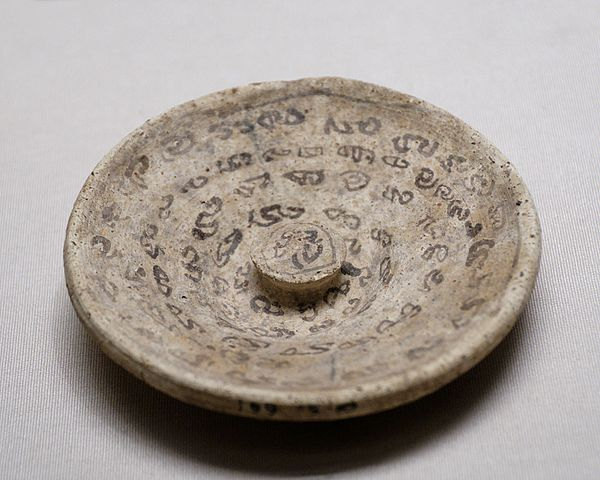
\includegraphics[scale=0.82]{magic_lid.jpg}
  \end{figure}
\end{frame}

\end{document}
